\section{Hausdorffova míra a Hausdorffova dimenze}\label{sec:hausdorffova-mira-dimenze}

Způsobů,~jak definovat dimenzi je celá řada. Zatím jsme společně prozkoumali box-counting dimenzi (resp. některá její pojetí),~avšak lze najít více způsobů její definice\footnote{Některé další jsou sepsány např. v~\citep[str. 40]{Falconer2014}.}. Pravděpodobně však nejstarším exemplářem svého druhu je tzv. \emph{Hausdorffova dimenze} a s~ní související \emph{Hausdorffova míra},~které hrají ve fraktální geometrii velice podstatnou roli. Stále se však budeme zabývat pouze množinami v~$\R^n$. Jsou pojmenovány po německém matematikovi \name{Felixi Hausdorffovi} (1868--1942).
\begin{figure}[h]
    \centering
    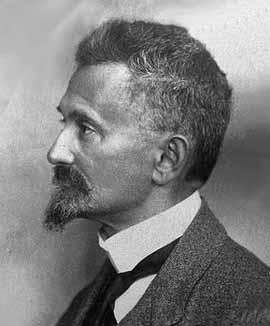
\includegraphics[width=0.4\textwidth]{felix-hausdorff.jpg}
    \caption[Felix Hausdorff,~1868--1942]{Felix Hausdorff\footnote{Převzato z~\cite{OConnorHausdorff2025}},~1868--1942}
    \label{fig:felix-hausdorff}
\end{figure}

\subsection{Definice Hausdorffovy míry}\label{subsec:hd-mira-definice}

\begin{definition}\label{def:hd-mira-delta}
    Nechť je dána množina $F\subseteq\R^n$ a $s>0$. Pak pro každé $\delta>0$ definujeme zobrazení
    \[\hausdorffdeltameasure{s}{\delta}(F)=\inf\set{\sum_{i=1}^{\infty}(\diam{F_i})^s\;\middle|\;F\subseteq\bigcup_{i=1}^\infty F_i\;,\;\diam{F_j}\leqslant\delta\;\text{pro}\;j\in\N}.\]
\end{definition}
Na první pohled si lze všimnout,~že pro $0<\delta_1<\delta_2$ je $\hausdorffdeltameasure{s}{\delta_1}(F)\leqslant\hausdorffdeltameasure{s}{\delta_2}(F)$. Jinými slovy,~pro $\delta\to 0$ hodnota $\hausdorffdeltameasure{s}{\delta}(F)$ klesá. Toto není nikterak těžké si rozmyslet,~neboť pro $\delta_1<\delta_2$ existuje $\delta_1$-pokrytí $\mathcal{F}_1$,~takové,~že je podpokrytím $\delta_2$-pokrytí $\mathcal{F}_2$ množiny $F$,~tedy $\mathcal{F}_1\subseteq\mathcal{F}_2$. To znamená,~že
\begin{align*}
    \hausdorffdeltameasure{s}{\delta_1}(F)&=\inf\set{\sum_{U\in\mathcal{F}_1}(\diam{U})^s\;\middle|\;\text{$\mathcal{F}_1$ je $\delta_1$-pokrytí}}\\
    &\leqslant\inf\set{\sum_{U\in\mathcal{F}_2}(\diam{U})^s\;\middle|\;\text{$\mathcal{F}_2$ je $\delta_2$-pokrytí}}=\hausdorffdeltameasure{s}{\delta_2}(F).
\end{align*}
Zároveň je z~definice \ref{def:hd-mira-delta} zjevné,~že $\mathcal{H}_\delta^s(F)\geqslant 0$.
\begin{definition}[Hausdorffova míra]\label{def:hausdorffova-mira}
    Nechť $F\subseteq\R^n$. Pak pro množinu $F$ definujeme \emph{$s$-dimenzionální Hausdorffovu míru}\index{míra!Hausdorffova} jako
    \[\hausdorffmeasure{s}(F)=\lim_{\delta\to 0}\hausdorffdeltameasure{s}{\delta}(F).\]
\end{definition}
Z přechodzího je zjevné,~že limita v~definici \ref{def:hausdorffova-mira} vždy existuje.

Bude dobré se přesvědčit,~že je Hausdorffova míra mírou ve smyslu definice \ref{def:prostor-s-mirou}. Začneme však otázkou. \emph{Na jaké množině je potřeba Hausdorffovu míru $\hausdorffmeasure{s}$ uvažovat?} Odpověď nám poskytují tzv. \emph{borelovské množiny}\index{množina!borelovská},~které jsou pojmenovány po francouzském matematikovi \name{Émile Borelovi} (1871--1956).
\begin{figure}[h]
    \centering
    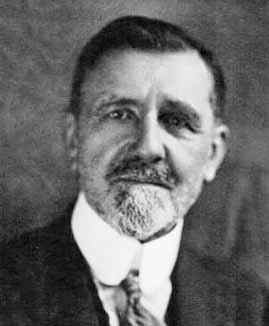
\includegraphics[width=0.4\textwidth]{Emile-Borel.jpeg}
    \caption[Émile Borel,~1871--1956]{Émile Borel\footnote{Převzato z~\cite{OConnorBorel2025}},~1871--1956}
\end{figure}
Borelovské množiny hrají podstatnou roli v~tzv. \emph{Deskriptivní teorii množin}. Nebudeme si zde vykládat všechny souvislosti,~vystačíme si se základem. Takto nazýváme všechny množiny,~které lze získat operacemi spočetného sjednocení a průniku otevřených množin z~$X$. Označme systém takových množin jako $\mathcal{B}$. Na tomto základě pak definujeme tzv. \emph{$\sigma$-algebru borelovských množin na $X$}:
\[\borelsigmaalgebra(X)=\bigcap_{\substack{\mathcal{F}\supseteq\mathcal{B}\\\text{$\mathcal{F}$ je $\sigma$-algebra}}}\mathcal{F}.\]
Jinými slovy,~$\borelsigmaalgebra(X)$ je nejmenší $\sigma$-algebra generovaná\footnote{Obecně $\sigma$-algebra $\mathcal{A}$ je generovaná množinou $X$,~když
\[\mathcal{A}=\bigcap_{\substack{\mathcal{F}\supseteq X\\\text{$\mathcal{F}$ je $\sigma$-algebra}}}\mathcal{F}.\]
Tento fakt se někdy značí $\mathcal{A}=\sigma(X)$.} všemi otevřenými množinami z~$X$.

Nás speciálně bude zajímat $\sigma$-algebra $\borelsigmaalgebra(\R^n)$. Nejdříve si však dokážeme dvě pomocná lemmata.
\begin{remark}
    V případě práce s množinou $\R^n$ a Hausdorffovou mírou $\hausdorffmeasure{s}(F)$, resp. $\hausdorffdeltameasure{s}{\delta}(F)$, budeme vždy předpokládat, že $F\in\borelsigmaalgebra(\R^n)$.
\end{remark}
\begin{lemma}[$\sigma$-subaditivita Hausdorffovy míry]\label{lem:Hausdorffova-mira-subaditivita}
    Nechť jsou dány množiny $A_1,A_2,\ldots$,~kde $A_i\subseteq\R^n$ pro každé $i\in\N$. Pak pro každé $s\geqslant 0$ platí
    \[\hausdorffmeasure{s}\left(\bigcup_{i=1}^\infty A_i\right)\leqslant\sum_{i=1}^{\infty}\hausdorffmeasure{s}(A_i).\]
\end{lemma}
\begin{proof}
    Nechť $s\geqslant 0$. Pro každé $i\in\N$ a $\delta>0$ mějme pokrytí
    \[\mathcal{F}_i=\set{F_{i,1},F_{i,2},\dots}\]
    množiny $A_i$,~takové,~že pro každé $j\in\N$ a $\varepsilon$ platí
    \[\sum_{j=1}^{\infty}(\diam{F_{i,j}})^s\leqslant\hausdorffdeltameasure{s}{\delta}(A_i)+\dfrac{\varepsilon}{2^i}.\]
    Systém $\bigcup_{i=1}^\infty\mathcal{F}_i$ tedy tvoří $\delta$-pokrytí množiny $A=\bigcup_{i=1}^\infty A_i$. Celkově
    \begin{align*}
        \hausdorffdeltameasure{s}{\delta}\left(\bigcup_{i=1}^\infty A_i\right)&\leqslant\sum_{i,j\in\N}(\diam{F_{i,j}})^s=\sum_{i=1}^{\infty}\sum_{j=1}^{\infty}(\diam{F_{i,j}})^s\leqslant\sum_{i=1}^{\infty}\left(\hausdorffdeltameasure{s}{\delta}(A_i)+\dfrac{\varepsilon}{2^i}\right)\\
        &=\sum_{i=1}^{\infty}\hausdorffdeltameasure{s}{\delta}(A_i)+\varepsilon.
    \end{align*}
    Limitním přechodem $\delta\to 0$ a aplikací Leviho věty\footnote{\emph{Leviho věta o~záměně pořadí limity a lebesgueova integrálu} říká,~že je-li posloupnost nezáporných měřitelných funkcí $\set{f_n}_{n=1}^\infty$ neklesající,~tj.
    \[f_1\leqslant f_2\leqslant\dots\]
    na prostoru $(X,\mathcal{A},\mu)$ a zároveň $\lim_{n\to\infty}f_n(x)=f(x)$ pro každé $x\in X$,~pak
    \[\lim_{n\to\infty}\int_X f_n\dx[\mu]=\int_X \lim_{n\to\infty}f_n\dx[\mu].\]
    Zde je speciálně $\mu$ aritmetická míra $X=\N$,~a $f_n(i)$ lze volit např. $\hausdorffdeltameasure{s}{1/n}(A_i)$. Z~Heineho věty víme,~že
    \[\lim_{n\to\infty}\hausdorffdeltameasure{s}{1/n}(A_i)=\lim_{\delta\to 0}\hausdorffdeltameasure{s}{\delta}(A_i)=\hausdorffmeasure{s}(A_i).\]
    }
    dostáváme
    \begin{align*}
        \hausdorffmeasure{s}\left(\bigcup_{i=1}^\infty A_i\right)&=\lim_{\delta\to 0}\hausdorffdeltameasure{s}{\delta}\left(\bigcup_{i=1}^\infty A_i\right)\leqslant\lim_{\delta\to 0}\sum_{i=1}^{\infty}\hausdorffdeltameasure{s}{\delta}(A_i)+\varepsilon=\sum_{i=1}^{\infty}\lim_{\delta\to 0}\hausdorffdeltameasure{s}{\delta}(A_i)+\varepsilon\\
        &=\sum_{i=1}^{\infty}\hausdorffmeasure{s}(A_i)+\varepsilon.
    \end{align*} 
\end{proof}
\begin{lemma}\label{lem:hausdorffova-mira-sigma-aditivita-kladna-vzdalenost}
    Nechť $(X,\varrho)$ je metrický prostor,~kde $X\subseteq\R^n$,~a $A,B\subseteq X$,~takové,~že pro jejich vzdálenost platí $\varrho(A,B)>0$. Pak pro každé $s\geqslant 0$ platí
    \[\hausdorffmeasure{s}(A\cup B)=\hausdorffmeasure{s}(A)+\hausdorffmeasure{s}(B).\]
\end{lemma}
\begin{proof}
    Nerovnost $\hausdorffmeasure{s}(A\cup B)\leqslant\hausdorffmeasure{s}(A)+\hausdorffmeasure{s}(B)$ je zřejmá ze $\sigma$-subaditivity Hausdorffovy míry (viz lemma \ref{lem:Hausdorffova-mira-subaditivita}).

    Bez újmy na obecnosti předpokládejme,~že $\hausdorffmeasure{s}(A\cup B)<\infty$. Zvolme $\delta$-pokrytí $\mathcal{F}=\set{F_1,F_2,\ldots}$ množiny $A\cup B$,~takové,~že pro každé $\varepsilon>0$ je
    \[\sum_{i=1}^{\infty}\hausdorffmeasure{s}(F_i)\leqslant\hausdorffmeasure{s}(A\cup B)+\varepsilon.\]
    Opět bez újmy na obecnosti lze předpokládat,~že pro každé $i\in\N$ je $\diam{F_i}<\varrho(A,B)$. V~opačném případě bychom $F_i$ pokryli množnami s~menším průměrem. Z~toho pak plyne,~že každá z~množin $F_i$ má neprázdný průnik s~nejvýše jednou z~množin $A,B$,~tzn. z~pokrytí $\mathcal{F}$ lze vybrat dvě disjunktní podpokrytí množiny $A$,~resp. množiny $B$. Tedy celkově s~užitím předchozího lemmatu \ref{lem:Hausdorffova-mira-subaditivita} máme
    \begin{align*}
        \hausdorffmeasure{s}(A)+\hausdorffmeasure{s}(B)&\leqslant\hausdorffmeasure{s}\left(\bigcup_{\substack{i\in\N\\ A\cap F_i\neq\emptyset}}F_i\right)+\hausdorffmeasure{s}\left(\bigcup_{\substack{i\in\N\\ B\cap F_i\neq\emptyset}}F_i\right)\\
        &\leqslant\sum_{\substack{i\in\N\\ A\cap F_i\neq\emptyset}}\hausdorffmeasure{s}(F_i)+\sum_{\substack{i\in\N\\ B\cap F_i\neq\emptyset}}\hausdorffmeasure{s}(F_i)\\
        &\leqslant\sum_{i=1}^{\infty}\hausdorffmeasure{s}(F_i)\leqslant\hausdorffmeasure{s}(A\cup B)+\varepsilon.
    \end{align*}
\end{proof}
\begin{lemma}\label{lem:hausdorffova-mira-sigma-aditivita-temer-disjunktni}
    Nechť $(X,\varrho)$ je metrický prostor a $A_1,A_2,\ldots$ jsou po dvou téměř disjunktní množiny o~průměru nejvýše $\delta>0$,~přičemž $A_i\subseteq X$ pro každé $i\in\N$. Pak pro každé $s\geqslant 0$ platí
    \[\hausdorffmeasure{s}\left(\bigcup_{i=1}^\infty A_i\right)=\sum_{i=1}^{\infty}\hausdorffmeasure{s}(A_i).\]
\end{lemma}
\begin{proof}
    Ze $\sigma$-subaditivity víme,~že platí $\hausdorffmeasure{s}\left(\bigcup_{i=1}^\infty A_i\right)\leqslant\sum_{i=1}^{\infty}\hausdorffmeasure{s}(A_i)$. Bez újmy na obecnosti předpokládejme,~že $\hausdorffmeasure{s}\left(\bigcup_{i=1}^\infty A_i\right)<\infty$. Jako první položíme $N=\set{i\in\N\mid \interior{A_i}\neq\emptyset}$. Pak pro každou množinu $A_i$,~kde $i\in N$,~existuje množina $B_i$,~taková,~že $B_i\subseteq\interior{A_i}$ a zároveň
    \[\hausdorffmeasure{s}(B_i)\geqslant\hausdorffmeasure{s}(A_i)-\dfrac{\varepsilon}{2^i}.\]
    Pro každé $i,j\in N$ tedy platí,~že $\varrho(B_i,B_j)>0$. Pro každé $n\in\N$ zároveň platí,~že
    \[\bigcup_{i=1}^\infty A_i\supseteq\bigcup_{\substack{j\in N\\j\leqslant n}}B_j.\]
    Tedy podle lemmatu \ref{lem:hausdorffova-mira-sigma-aditivita-kladna-vzdalenost} je
    \begin{align*}
        \hausdorffmeasure{s}\left(\bigcup_{i=1}^\infty A_i\right)&\geqslant\hausdorffmeasure{s}\left(\bigcup_{\substack{j\in N\\j\leqslant n}}B_i\right)=\sum_{\substack{i\in N\\i\geqslant n}}\hausdorffmeasure{s}(B_i)=\sum_{i=1}^{n}\hausdorffmeasure{s}(B_i)\\
        &\geqslant\sum_{i=1}^{n}\left(\hausdorffmeasure{s}(A_i)-\dfrac{\varepsilon}{2^i}\right)=\sum_{i=1}^{n}\hausdorffmeasure{s}(A_i)-\varepsilon.
    \end{align*}
    U~třetí rovnosti jsme přidali množiny s~nulovou mírou. Pro $n\to\infty$ dostáváme
    \[\hausdorffmeasure{s}\left(\bigcup_{i=1}^\infty A_i\right)\geqslant\sum_{i=1}^{\infty}\hausdorffmeasure{s}(A_i)-\varepsilon.\]
\end{proof}
\begin{theorem}\label{thm:hausdorffova-mira-je-mira}
    Trojice $(\R^n,\borelsigmaalgebra(\R^n),\hausdorffmeasure{s})$,~kde $s\geqslant 0$,~tvoří prostor s~mírou.
\end{theorem}
Věta \ref{thm:hausdorffova-mira-je-mira} říká,~že omezíme-li se na $\sigma$-algebru borelovských množin,~pak $\hausdorffmeasure{s}$ je skutečně mírou.
\begin{proof}
    Fakt,~že $\hausdorffmeasure{s}(\emptyset)=0$ je zjevný. Stačí zvolit pokrytí množinami s~nulovým průměrem,~tedy např. prázdnými množinami. Platnost druhé vlastnosti plyne z~lemmatu \ref{lem:hausdorffova-mira-sigma-aditivita-temer-disjunktni}.
\end{proof}

Nyní již můžeme zobrazení $\hausdorffmeasure{s}$ nazývat mírou oprávněně. Pojďme se podívat na nějaké příklady.
\begin{example}
    Pro $s=0$ představuje zobrazení $\hausdorffmeasure{s}$ obyčejnou aritmetickou míru\index{míra!aritmetická},~tzn. pro konečnou množinu $A\subseteq\R^n$ je $\hausdorffmeasure{0}(A)=|A|$. Toto není těžké ukázat. Mějme množinu $A=\set{x_1,x_2,\ldots,x_n}$. Zvolíme-li
    \[\delta<\dfrac{1}{2}\cdot\min\set{\varrho_e(x_i,x_j)\mid 1\leqslant i,j\leqslant n},\]
    pak pro $\delta$-pokrytí $\mathcal{F}=\set{F_1,F_2,\ldots,F_n}$ takové,~že $x_i\in F_i$ pro každé $i$ máme
    \[\sum_{i=1}^{n}(\diam{F_i})^0=\sum_{i=1}^{n}1=n.\]
    Není těžké si rozmyslet,~že $n$ je nejmenší počet množin o~průměru nejvýše $\delta$,~takových,~aby pokrývaly množinu $A$. Zároveň pro libovolné $\varepsilon>0$ je potřeba nejvýše $n$-koulí o~poloměru $\varepsilon/2$ se středy v~$x_i$ pro pokrytí $A$. Tzn.~$\hausdorffmeasure{0}(A)=|A|=n$.
\end{example}

V rámci tohoto textu jsme se již zabývali jiným typem míry a to tzv. \emph{lebesgueovou mírou} (viz sekce \ref{sec:lebesgueova-mira}). Ta pro nás hrála důležitou roli v jednom možném pojetí \emph{box-counting dimenze} (viz sekce \ref{sec:box-counting-dimenze}). Lze ukázat, že pro množinu $F\subseteq\R^n$ je
\[\hausdorffmeasure{n}(F)=\dfrac{1}{v_n}\lebesguemeasure{n}(F),\]
kde $v_n$ je objem (míra) jednotkové koule v $\R^n$. Čtenář snad promine, že tento fakt zde ponecháme bez důkazu. \citep[str. 45]{Falconer2014}

\subsection{Vlastnosti Hausdorffovy míry}\label{subsec:vlastnosti-hausdorffovy-miry}

Na chvíli se ještě zastavíme u vlastností Hausdorffovy míry. Již jsme společně dokázali, že Hausdorffova míra je skutečně mírou, tzn. splňuje všechny základní vlastnosti, které jsme si představili ve větě \ref{thm:mira-vlastnosti} (viz sekce \ref{sec:prostory-s-mirou}). V tomto ohledu tedy netřeba již nic dalšího dokazovat. Nicméně podobně jako v případě \emph{box-counting dimenze} (viz podsekce \ref{subsec:vlastnosti-bc-dimenze}) se i zde podíváme, jak se Hausdorffova míra chová vůči \emph{lipschitzovským zobrazením}\index{zobrazení!lipschitzovské}.
\begin{theorem}
    Nechť $F\subseteq\R^n$ a zobrazení $\mapping{f}{F}{\R^n}$ je lipschitzovské\footnote{Tvrzení lze zformulovat obecněji pro tzv. \emph{hölderovská zobrazení}\index{zobrazení!hölderovské}, tedy zobrazení $f$ splnující
    \[\varrho(f(x),f(y))\leqslant K(\varrho(x,y))^\alpha.\]
    kde $\alpha>0$. Pak pro $F\subseteq\R^n$ platí
    \[\hausdorffmeasure{s/\alpha}(f(F))\leqslant K^{s/\alpha}\hausdorffmeasure{s}(F).\]
    My si však vystačíme se speciálním případem.} s konstantou $K>0$. Pak pro každé $s\geqslant 0$ platí
    \[\hausdorffmeasure{s}(f(F))\leqslant K^s\hausdorffmeasure{s}(F).\]
\end{theorem}
\begin{proof}
    Nechť $\mathcal{F}=\set{F_1,F_2,\ldots}$ je $\delta$-pokrytí $F$. Pak
    \[\diam(f(F\cap F_i))\leqslant K\diam(F\cap F_i)\leqslant K\diam{F_i},\]
    což znamená, že $\mathcal{G}=\set{F\cap F_1,F\cap F_2,\ldots}$ je $K\delta$-pokrytí $f(F)$. Z toho plyne, že
    \[\sum_{i=1}^{\infty}(\diam(F\cap F_i))^s\leqslant K^s\sum_{i=1}^{\infty}(\diam{F_i})^s\]
    a tedy $\hausdorffdeltameasure{s}{K\delta}(f(F))\leqslant K^s\hausdorffdeltameasure{s}{\delta}(F)$. Pro $\delta\to 0$ máme požadovaný výsledek.
\end{proof}

\subsection{Hausdorffova dimenze}\label{subsec:hausdorffova-dimenze}

Středobodem této sekce je tzv. \emph{Hausdorffova dimenze}\index{dimenze!Hausdorffova}. Na úvod si dokážeme jedno jednoduché tvrzení týkající se Hausdorffovy míry.
\begin{theorem}\label{thm:hodnoty-hausdorffovy-miry}
    Nechť $0\leqslant s<t<\infty$ a $F\subseteq X$. Pak platí:
    \begin{enumerate}[label=(\roman*)]
        \item\label{thm:hd-dimenze-konecna} $\hausdorffmeasure{s}(F)<\infty\implies\hausdorffmeasure{t}(F)=0$,
        \item\label{thm:hd-dimenze-nekonecno} $\hausdorffmeasure{t}(F)>0\implies\hausdorffmeasure{s}(F)=\infty$.
    \end{enumerate}
\end{theorem}
\begin{proof}
    Mějme $\delta$-pokrytí $\mathcal{F}=\set{F_1,F_2,\ldots}$,~takové,~že
    \[\sum_{i=1}^{\infty}(\diam{F_i})^s\leqslant\hausdorffdeltameasure{s}{\delta}(F)+\varepsilon\;,\;\varepsilon>0.\]
    Pak
    \[\hausdorffdeltameasure{t}{\delta}(F)\leqslant\sum_{i=1}^{\infty}(\diam{F_i})^t\leqslant\delta^{t-s}\sum_{i=1}^{\infty}(\diam{F_i})^s\leqslant\delta^{t-s}(\hausdorffdeltameasure{s}{\delta}(F)+\varepsilon).\]
    Tzn.~$\hausdorffdeltameasure{t}{\delta}(F)\leqslant\delta^{t-s}\hausdorffdeltameasure{s}{\delta}(F)$. Pro $\delta\to 0$ dostaneme body \ref{thm:hd-dimenze-konecna} a \ref{thm:hd-dimenze-nekonecno}.
\end{proof}
(Převzato z~\citep[str. 68]{Mattila1995}.)

Z věty \ref{thm:hodnoty-hausdorffovy-miry} lze vidět,~že Hausdorffova míra dává smysl jen pro určitou hodnotu $s$. Pro "příliš velké" $s$ bude hodnota vždy $0$,~naopak pro "moc malé" $s$ bude jeho hodnota rovna $\infty$ (viz obrázek \ref{fig:hausdorffova-dimenze-graf}).
\begin{figure}[h]
    \centering
    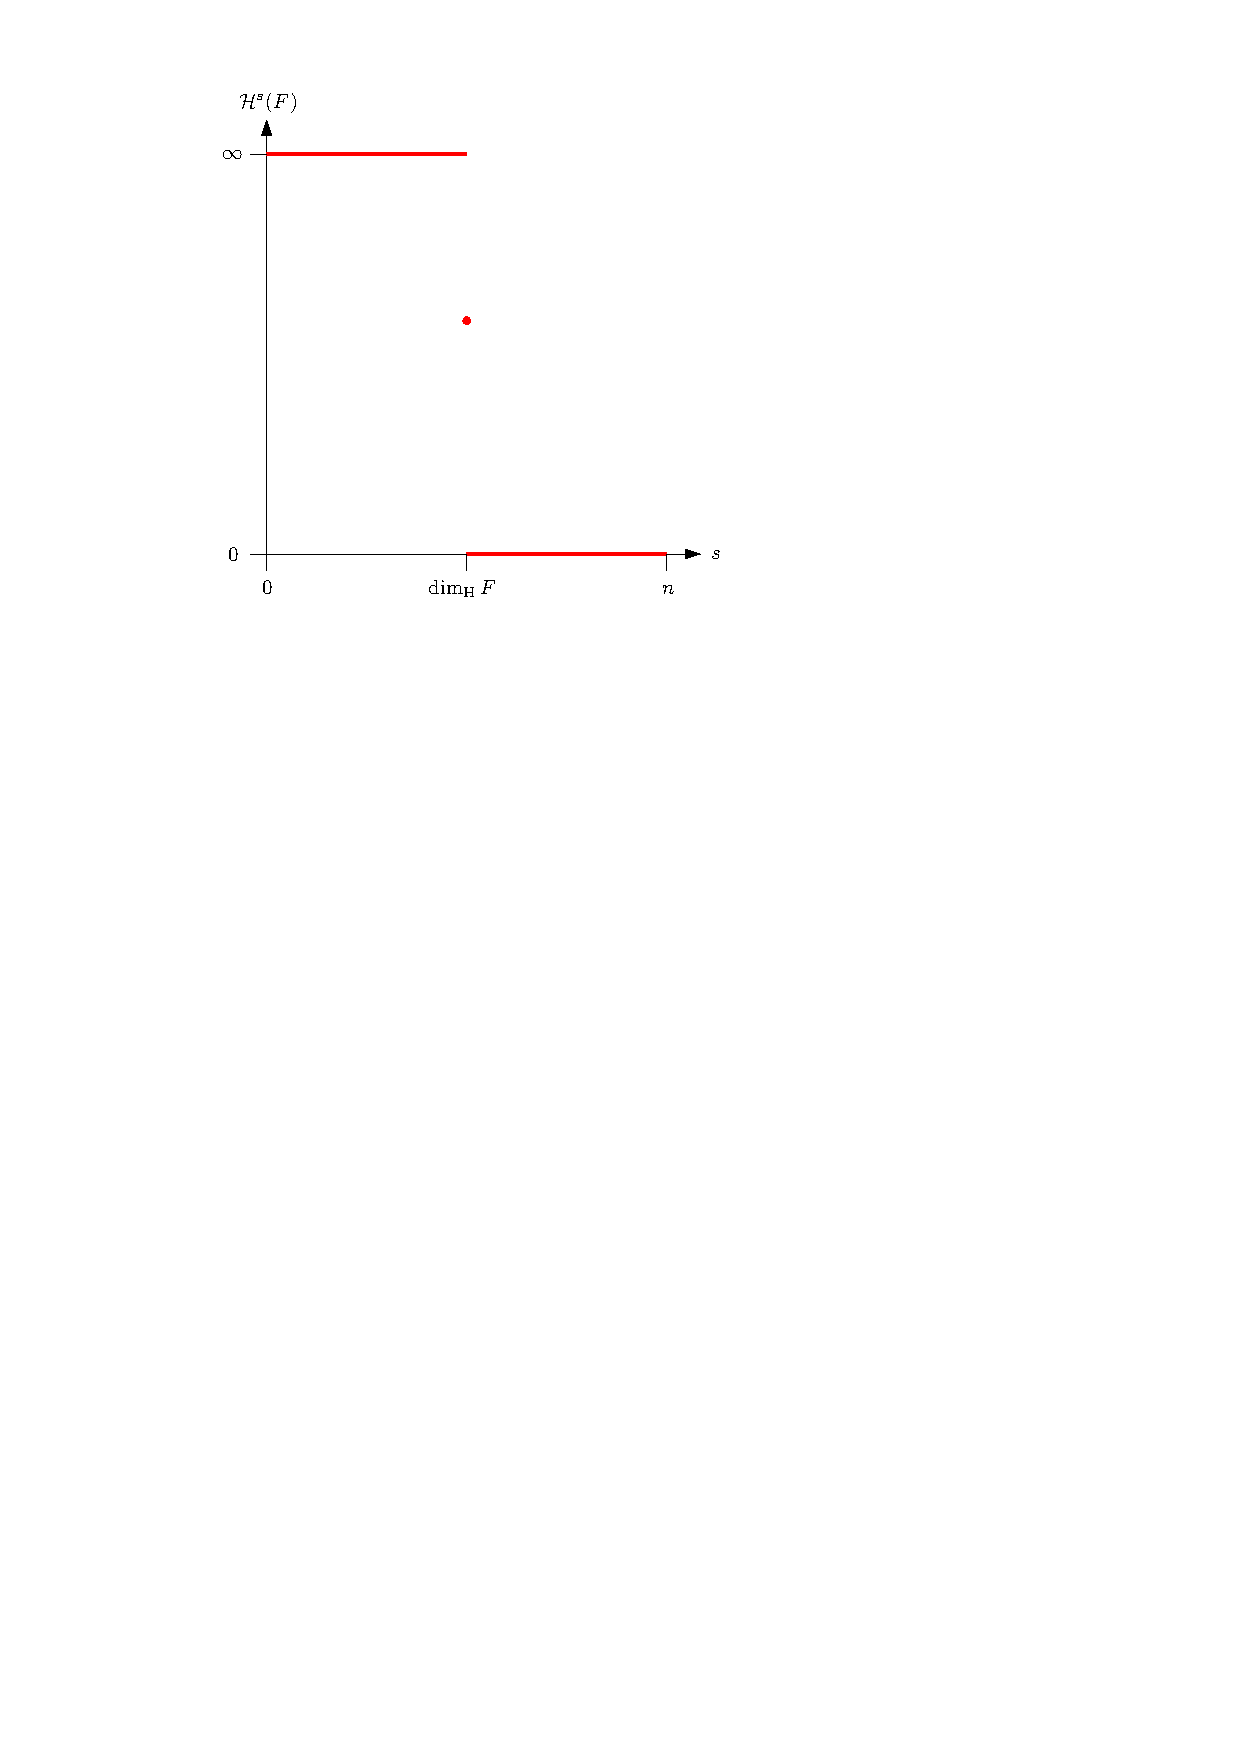
\includegraphics{ch02-hausdorffova-dimenze-graf.pdf}
    \caption{Graf funkce $f(s)=\hausdorffmeasure{s}(F)$,~kde $F\subseteq\R^n$.}
    \label{fig:hausdorffova-dimenze-graf}
\end{figure}
Této kritické hodnotě $s$ říkáme \emph{Hausdorffova dimenze}\index{dimenze!Hausdorffova}.
\begin{definition}[Hausdorffova dimenze]\label{def:hausdorffova-dimenze}
    Nechť $F\subseteq\R^n$. Hausdorffovou dimenzí\footnote{Též někdy nazývaná \emph{Hausdorffova-Bezikovičova dimenze}\index{dimenze!Hausdorffova-Bezikovičkova}. }\index{dimenze!Hausdorffova} množiny $F$ nazveme hodnotu
    \[\dimH{F}=\inf\set{s\geqslant 0\mid\hausdorffmeasure{s}(F)=0}=\sup\set{s\geqslant 0\mid\hausdorffmeasure{s}(F)=\infty}.\]
\end{definition}
Hodnota $\hausdorffmeasure{s}(F)$ pro $s=\dimH{F}$ může být různá,~tzn. může platit,~že $\hausdorffmeasure{s}(F)=\infty$,~$\hausdorffmeasure{s}(F)=0$ a nebo se může jednat o~konečné nenulové číslo,~tj. $0<\hausdorffmeasure{s}(F)<\infty$.